\documentclass[]{article}
\usepackage{lmodern}
\usepackage{amssymb,amsmath}
\usepackage{ifxetex,ifluatex}
\usepackage{fixltx2e} % provides \textsubscript
\ifnum 0\ifxetex 1\fi\ifluatex 1\fi=0 % if pdftex
  \usepackage[T1]{fontenc}
  \usepackage[utf8]{inputenc}
\else % if luatex or xelatex
  \ifxetex
    \usepackage{mathspec}
  \else
    \usepackage{fontspec}
  \fi
  \defaultfontfeatures{Ligatures=TeX,Scale=MatchLowercase}
\fi
% use upquote if available, for straight quotes in verbatim environments
\IfFileExists{upquote.sty}{\usepackage{upquote}}{}
% use microtype if available
\IfFileExists{microtype.sty}{%
\usepackage{microtype}
\UseMicrotypeSet[protrusion]{basicmath} % disable protrusion for tt fonts
}{}
\usepackage[margin=1in]{geometry}
\usepackage{hyperref}
\hypersetup{unicode=true,
            pdftitle={Simple Descriptive Techniques for Time Series Analysis},
            pdfauthor={Amir R},
            pdfborder={0 0 0},
            breaklinks=true}
\urlstyle{same}  % don't use monospace font for urls
\usepackage{color}
\usepackage{fancyvrb}
\newcommand{\VerbBar}{|}
\newcommand{\VERB}{\Verb[commandchars=\\\{\}]}
\DefineVerbatimEnvironment{Highlighting}{Verbatim}{commandchars=\\\{\}}
% Add ',fontsize=\small' for more characters per line
\usepackage{framed}
\definecolor{shadecolor}{RGB}{248,248,248}
\newenvironment{Shaded}{\begin{snugshade}}{\end{snugshade}}
\newcommand{\AlertTok}[1]{\textcolor[rgb]{0.94,0.16,0.16}{#1}}
\newcommand{\AnnotationTok}[1]{\textcolor[rgb]{0.56,0.35,0.01}{\textbf{\textit{#1}}}}
\newcommand{\AttributeTok}[1]{\textcolor[rgb]{0.77,0.63,0.00}{#1}}
\newcommand{\BaseNTok}[1]{\textcolor[rgb]{0.00,0.00,0.81}{#1}}
\newcommand{\BuiltInTok}[1]{#1}
\newcommand{\CharTok}[1]{\textcolor[rgb]{0.31,0.60,0.02}{#1}}
\newcommand{\CommentTok}[1]{\textcolor[rgb]{0.56,0.35,0.01}{\textit{#1}}}
\newcommand{\CommentVarTok}[1]{\textcolor[rgb]{0.56,0.35,0.01}{\textbf{\textit{#1}}}}
\newcommand{\ConstantTok}[1]{\textcolor[rgb]{0.00,0.00,0.00}{#1}}
\newcommand{\ControlFlowTok}[1]{\textcolor[rgb]{0.13,0.29,0.53}{\textbf{#1}}}
\newcommand{\DataTypeTok}[1]{\textcolor[rgb]{0.13,0.29,0.53}{#1}}
\newcommand{\DecValTok}[1]{\textcolor[rgb]{0.00,0.00,0.81}{#1}}
\newcommand{\DocumentationTok}[1]{\textcolor[rgb]{0.56,0.35,0.01}{\textbf{\textit{#1}}}}
\newcommand{\ErrorTok}[1]{\textcolor[rgb]{0.64,0.00,0.00}{\textbf{#1}}}
\newcommand{\ExtensionTok}[1]{#1}
\newcommand{\FloatTok}[1]{\textcolor[rgb]{0.00,0.00,0.81}{#1}}
\newcommand{\FunctionTok}[1]{\textcolor[rgb]{0.00,0.00,0.00}{#1}}
\newcommand{\ImportTok}[1]{#1}
\newcommand{\InformationTok}[1]{\textcolor[rgb]{0.56,0.35,0.01}{\textbf{\textit{#1}}}}
\newcommand{\KeywordTok}[1]{\textcolor[rgb]{0.13,0.29,0.53}{\textbf{#1}}}
\newcommand{\NormalTok}[1]{#1}
\newcommand{\OperatorTok}[1]{\textcolor[rgb]{0.81,0.36,0.00}{\textbf{#1}}}
\newcommand{\OtherTok}[1]{\textcolor[rgb]{0.56,0.35,0.01}{#1}}
\newcommand{\PreprocessorTok}[1]{\textcolor[rgb]{0.56,0.35,0.01}{\textit{#1}}}
\newcommand{\RegionMarkerTok}[1]{#1}
\newcommand{\SpecialCharTok}[1]{\textcolor[rgb]{0.00,0.00,0.00}{#1}}
\newcommand{\SpecialStringTok}[1]{\textcolor[rgb]{0.31,0.60,0.02}{#1}}
\newcommand{\StringTok}[1]{\textcolor[rgb]{0.31,0.60,0.02}{#1}}
\newcommand{\VariableTok}[1]{\textcolor[rgb]{0.00,0.00,0.00}{#1}}
\newcommand{\VerbatimStringTok}[1]{\textcolor[rgb]{0.31,0.60,0.02}{#1}}
\newcommand{\WarningTok}[1]{\textcolor[rgb]{0.56,0.35,0.01}{\textbf{\textit{#1}}}}
\usepackage{graphicx,grffile}
\makeatletter
\def\maxwidth{\ifdim\Gin@nat@width>\linewidth\linewidth\else\Gin@nat@width\fi}
\def\maxheight{\ifdim\Gin@nat@height>\textheight\textheight\else\Gin@nat@height\fi}
\makeatother
% Scale images if necessary, so that they will not overflow the page
% margins by default, and it is still possible to overwrite the defaults
% using explicit options in \includegraphics[width, height, ...]{}
\setkeys{Gin}{width=\maxwidth,height=\maxheight,keepaspectratio}
\IfFileExists{parskip.sty}{%
\usepackage{parskip}
}{% else
\setlength{\parindent}{0pt}
\setlength{\parskip}{6pt plus 2pt minus 1pt}
}
\setlength{\emergencystretch}{3em}  % prevent overfull lines
\providecommand{\tightlist}{%
  \setlength{\itemsep}{0pt}\setlength{\parskip}{0pt}}
\setcounter{secnumdepth}{0}
% Redefines (sub)paragraphs to behave more like sections
\ifx\paragraph\undefined\else
\let\oldparagraph\paragraph
\renewcommand{\paragraph}[1]{\oldparagraph{#1}\mbox{}}
\fi
\ifx\subparagraph\undefined\else
\let\oldsubparagraph\subparagraph
\renewcommand{\subparagraph}[1]{\oldsubparagraph{#1}\mbox{}}
\fi

%%% Use protect on footnotes to avoid problems with footnotes in titles
\let\rmarkdownfootnote\footnote%
\def\footnote{\protect\rmarkdownfootnote}

%%% Change title format to be more compact
\usepackage{titling}

% Create subtitle command for use in maketitle
\providecommand{\subtitle}[1]{
  \posttitle{
    \begin{center}\large#1\end{center}
    }
}

\setlength{\droptitle}{-2em}

  \title{Simple Descriptive Techniques for Time Series Analysis}
    \pretitle{\vspace{\droptitle}\centering\huge}
  \posttitle{\par}
    \author{Amir R}
    \preauthor{\centering\large\emph}
  \postauthor{\par}
    \date{}
    \predate{}\postdate{}
  

\begin{document}
\maketitle

Let's load some sample data

\begin{Shaded}
\begin{Highlighting}[]
\KeywordTok{load}\NormalTok{(}\StringTok{"TSsimple.RData"}\NormalTok{)}
\end{Highlighting}
\end{Shaded}

and examine its structure

\begin{Shaded}
\begin{Highlighting}[]
\NormalTok{blowfly<-}\KeywordTok{read.csv}\NormalTok{(}\StringTok{"blowfly.csv"}\NormalTok{, }\DataTypeTok{header=}\NormalTok{T) }\CommentTok{#delete later}
\KeywordTok{str}\NormalTok{(blowfly)}
\end{Highlighting}
\end{Shaded}

\begin{verbatim}
## 'data.frame':    361 obs. of  5 variables:
##  $ eggs       : int  0 0 0 0 2149 4627 4523 6030 2684 3373 ...
##  $ nonemerging: int  0 0 0 0 121 260 281 458 120 176 ...
##  $ emerging   : int  948 4 0 0 0 0 0 0 0 0 ...
##  $ deaths     : int  0 10 31 53 57 125 172 107 149 102 ...
##  $ total      : int  948 942 911 858 801 676 504 397 248 146 ...
\end{verbatim}

Time for a first look

\begin{Shaded}
\begin{Highlighting}[]
\KeywordTok{plot}\NormalTok{(blowfly}\OperatorTok{$}\NormalTok{total)}
\end{Highlighting}
\end{Shaded}

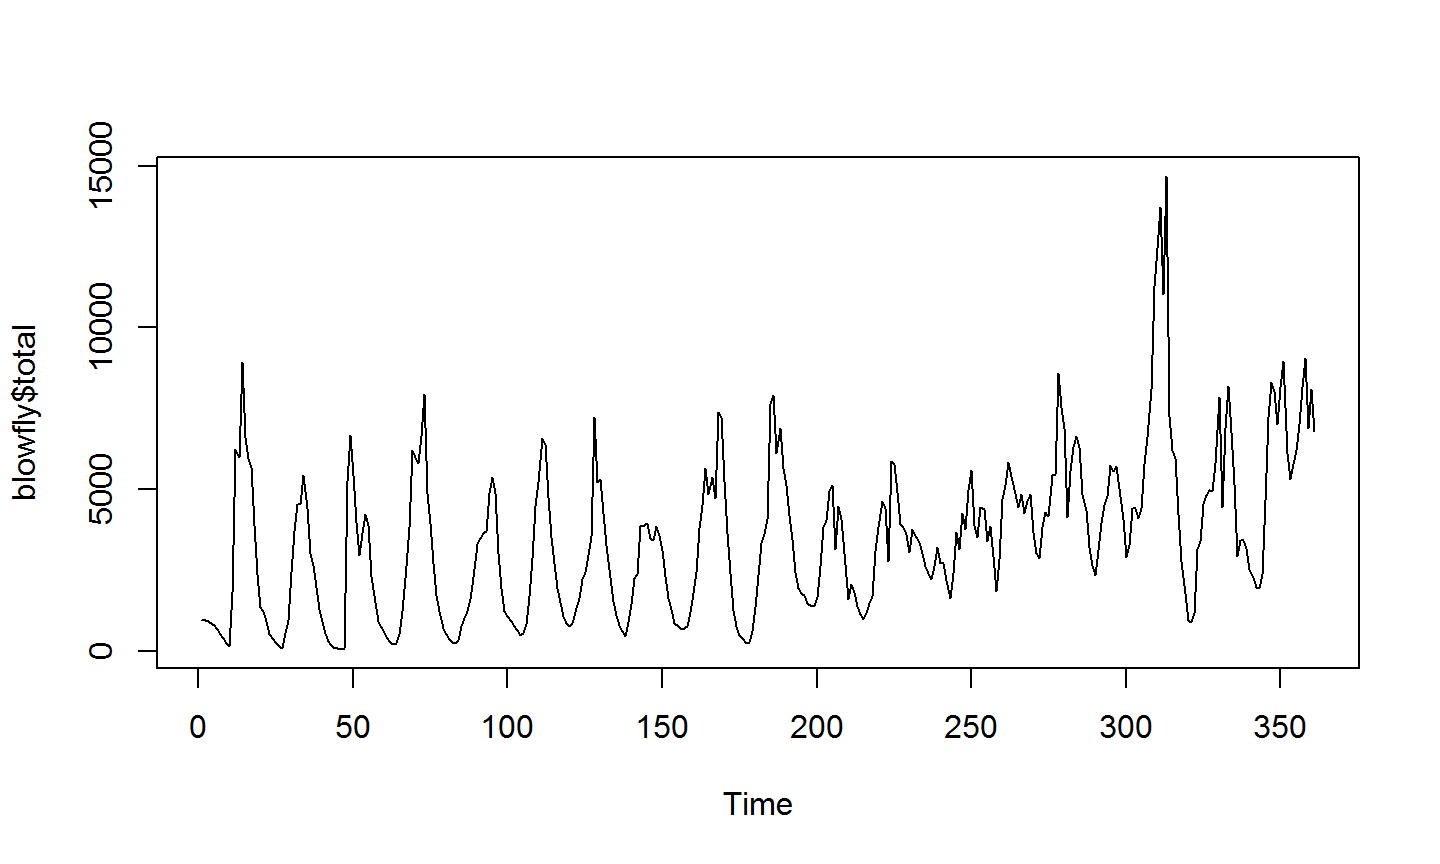
\includegraphics{simple_descriptive_techniques_files/figure-latex/unnamed-chunk-3-1.pdf}

\begin{Shaded}
\begin{Highlighting}[]
\KeywordTok{summary}\NormalTok{(blowfly}\OperatorTok{$}\NormalTok{total)}
\end{Highlighting}
\end{Shaded}

\begin{verbatim}
##    Min. 1st Qu.  Median    Mean 3rd Qu.    Max. 
##      60    1454    3350    3496    4897   14683
\end{verbatim}

and using a time series plotting method:

\begin{Shaded}
\begin{Highlighting}[]
\KeywordTok{plot.ts}\NormalTok{(blowfly}\OperatorTok{$}\NormalTok{total)}
\end{Highlighting}
\end{Shaded}

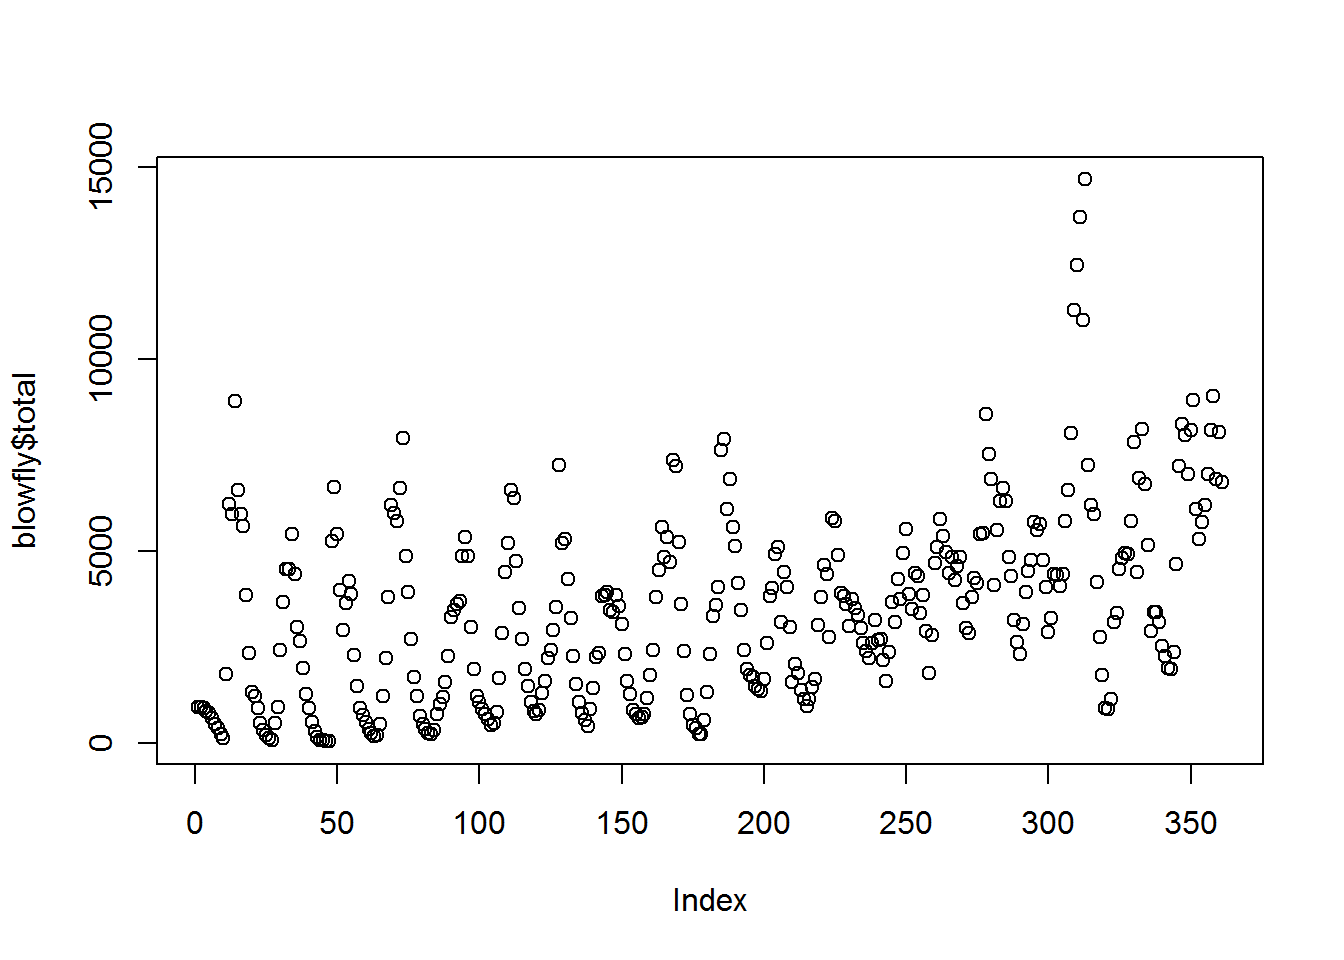
\includegraphics{simple_descriptive_techniques_files/figure-latex/unnamed-chunk-4-1.pdf}

\#The \texttt{ts} class

\texttt{plot.ts} plots the object as if it were of the special class of
R objects known simply as \emph{ts}

the \texttt{ts()} function is used to convert objects to the ts class

\begin{Shaded}
\begin{Highlighting}[]
\NormalTok{flies<-}\KeywordTok{ts}\NormalTok{(blowfly}\OperatorTok{$}\NormalTok{total)}
\KeywordTok{class}\NormalTok{(flies)}
\end{Highlighting}
\end{Shaded}

\begin{verbatim}
## [1] "ts"
\end{verbatim}

\begin{Shaded}
\begin{Highlighting}[]
\KeywordTok{typeof}\NormalTok{(flies)}
\end{Highlighting}
\end{Shaded}

\begin{verbatim}
## [1] "integer"
\end{verbatim}

many base/stats functions are actually designed for the `ts' class

\begin{Shaded}
\begin{Highlighting}[]
\KeywordTok{plot}\NormalTok{(flies)}
\end{Highlighting}
\end{Shaded}

\includegraphics{simple_descriptive_techniques_files/figure-latex/unnamed-chunk-6-1.pdf}

\begin{Shaded}
\begin{Highlighting}[]
\KeywordTok{plot}\NormalTok{(flies[}\DecValTok{1}\OperatorTok{:}\DecValTok{100}\NormalTok{])}
\end{Highlighting}
\end{Shaded}

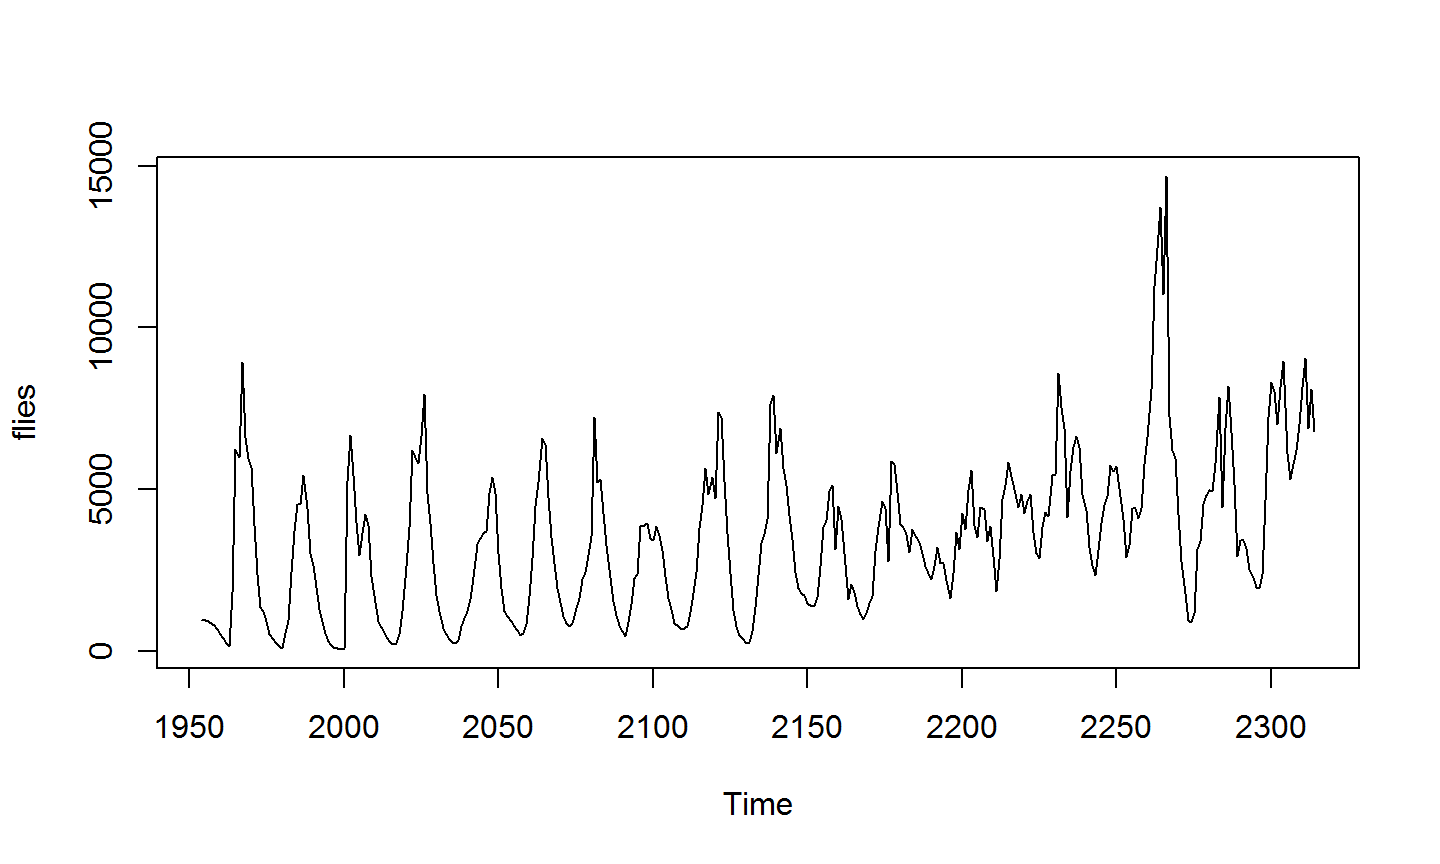
\includegraphics{simple_descriptive_techniques_files/figure-latex/unnamed-chunk-7-1.pdf}

\begin{Shaded}
\begin{Highlighting}[]
\KeywordTok{plot}\NormalTok{(flies[}\DecValTok{1}\OperatorTok{:}\DecValTok{300}\NormalTok{],flies[}\DecValTok{2}\OperatorTok{:}\DecValTok{301}\NormalTok{])}
\end{Highlighting}
\end{Shaded}

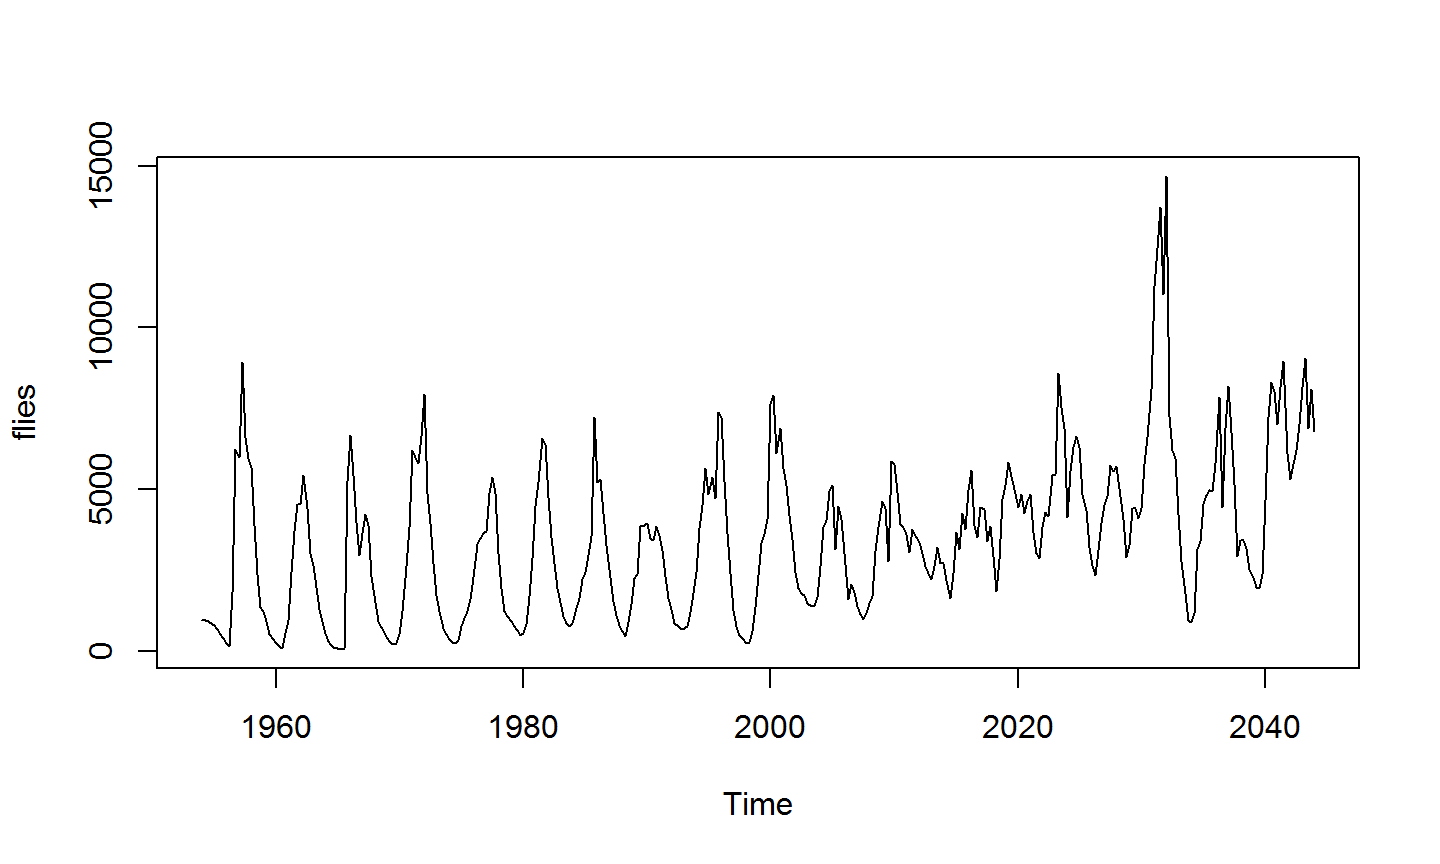
\includegraphics{simple_descriptive_techniques_files/figure-latex/unnamed-chunk-8-1.pdf}

\begin{Shaded}
\begin{Highlighting}[]
\KeywordTok{plot}\NormalTok{(flies[}\DecValTok{1}\OperatorTok{:}\DecValTok{300}\NormalTok{],flies[}\DecValTok{3}\OperatorTok{:}\DecValTok{302}\NormalTok{])}
\end{Highlighting}
\end{Shaded}

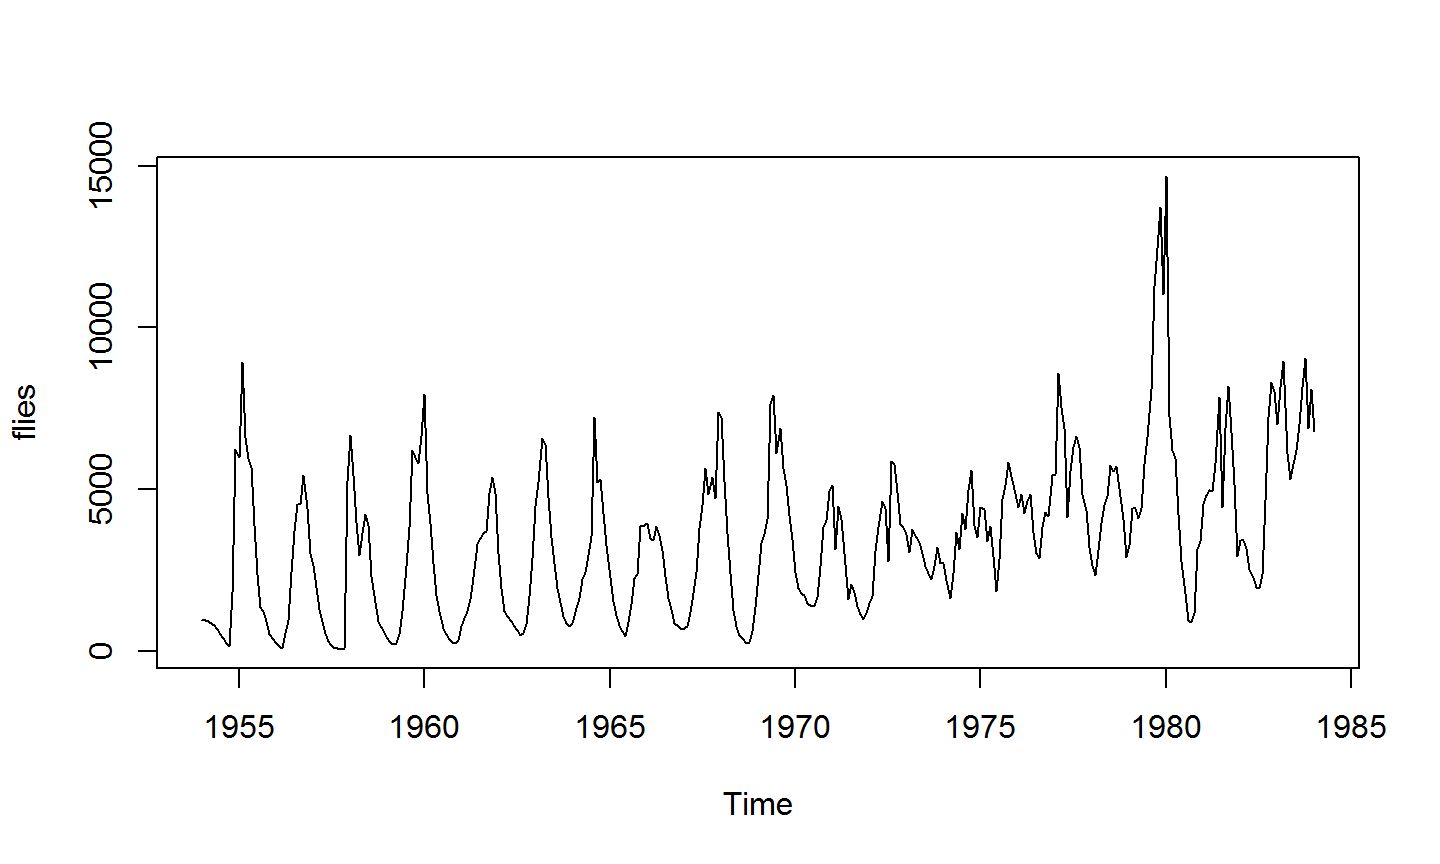
\includegraphics{simple_descriptive_techniques_files/figure-latex/unnamed-chunk-9-1.pdf}

\begin{Shaded}
\begin{Highlighting}[]
\KeywordTok{plot}\NormalTok{(flies[}\DecValTok{1}\OperatorTok{:}\DecValTok{300}\NormalTok{],flies[}\DecValTok{4}\OperatorTok{:}\DecValTok{303}\NormalTok{])}
\end{Highlighting}
\end{Shaded}

\includegraphics{simple_descriptive_techniques_files/figure-latex/unnamed-chunk-9-2.pdf}

\begin{Shaded}
\begin{Highlighting}[]
\KeywordTok{par}\NormalTok{(}\DataTypeTok{mfrow=}\KeywordTok{c}\NormalTok{(}\DecValTok{2}\NormalTok{,}\DecValTok{4}\NormalTok{))}
\KeywordTok{sapply}\NormalTok{(}\DecValTok{1}\OperatorTok{:}\DecValTok{8}\NormalTok{,}\ControlFlowTok{function}\NormalTok{ (x) }\KeywordTok{plot}\NormalTok{(flies[}\OperatorTok{-}\KeywordTok{c}\NormalTok{(}\DecValTok{1}\OperatorTok{:}\NormalTok{x)],flies[}\OperatorTok{-}\KeywordTok{c}\NormalTok{(}\DecValTok{361}\OperatorTok{:}\NormalTok{(}\DecValTok{361}\OperatorTok{-}\NormalTok{x}\OperatorTok{+}\DecValTok{1}\NormalTok{))]))}
\end{Highlighting}
\end{Shaded}

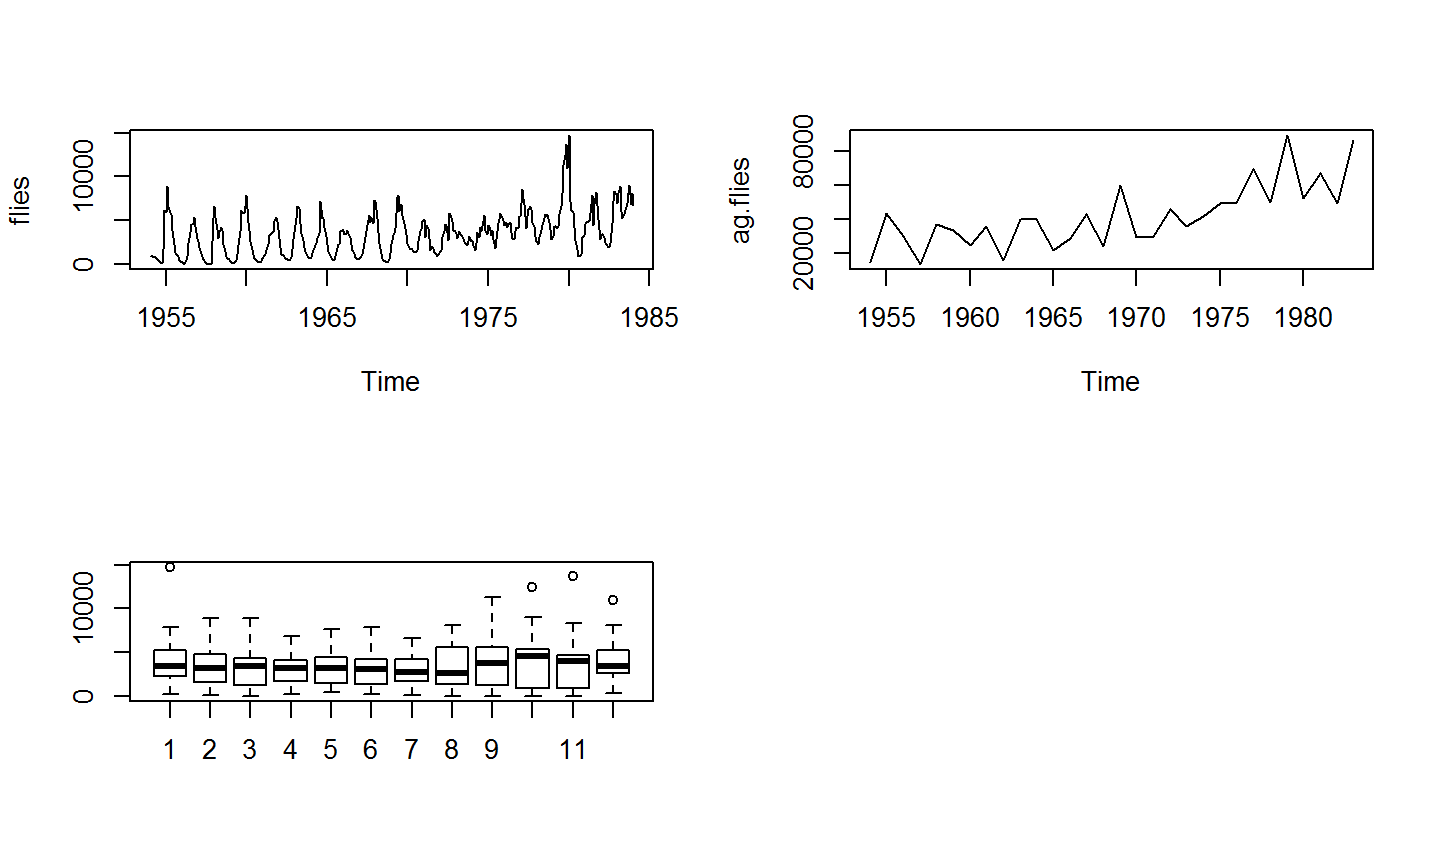
\includegraphics{simple_descriptive_techniques_files/figure-latex/unnamed-chunk-10-1.pdf}

\begin{verbatim}
## [[1]]
## NULL
## 
## [[2]]
## NULL
## 
## [[3]]
## NULL
## 
## [[4]]
## NULL
## 
## [[5]]
## NULL
## 
## [[6]]
## NULL
## 
## [[7]]
## NULL
## 
## [[8]]
## NULL
\end{verbatim}

\begin{Shaded}
\begin{Highlighting}[]
\KeywordTok{sapply}\NormalTok{(}\DecValTok{9}\OperatorTok{:}\DecValTok{16}\NormalTok{,}\ControlFlowTok{function}\NormalTok{ (x) }\KeywordTok{plot}\NormalTok{( flies[}\OperatorTok{-}\KeywordTok{c}\NormalTok{(}\DecValTok{1}\OperatorTok{:}\NormalTok{x)],flies[}\OperatorTok{-}\KeywordTok{c}\NormalTok{(}\DecValTok{361}\OperatorTok{:}\NormalTok{(}\DecValTok{361}\OperatorTok{-}\NormalTok{x}\OperatorTok{+}\DecValTok{1}\NormalTok{))]))}
\end{Highlighting}
\end{Shaded}

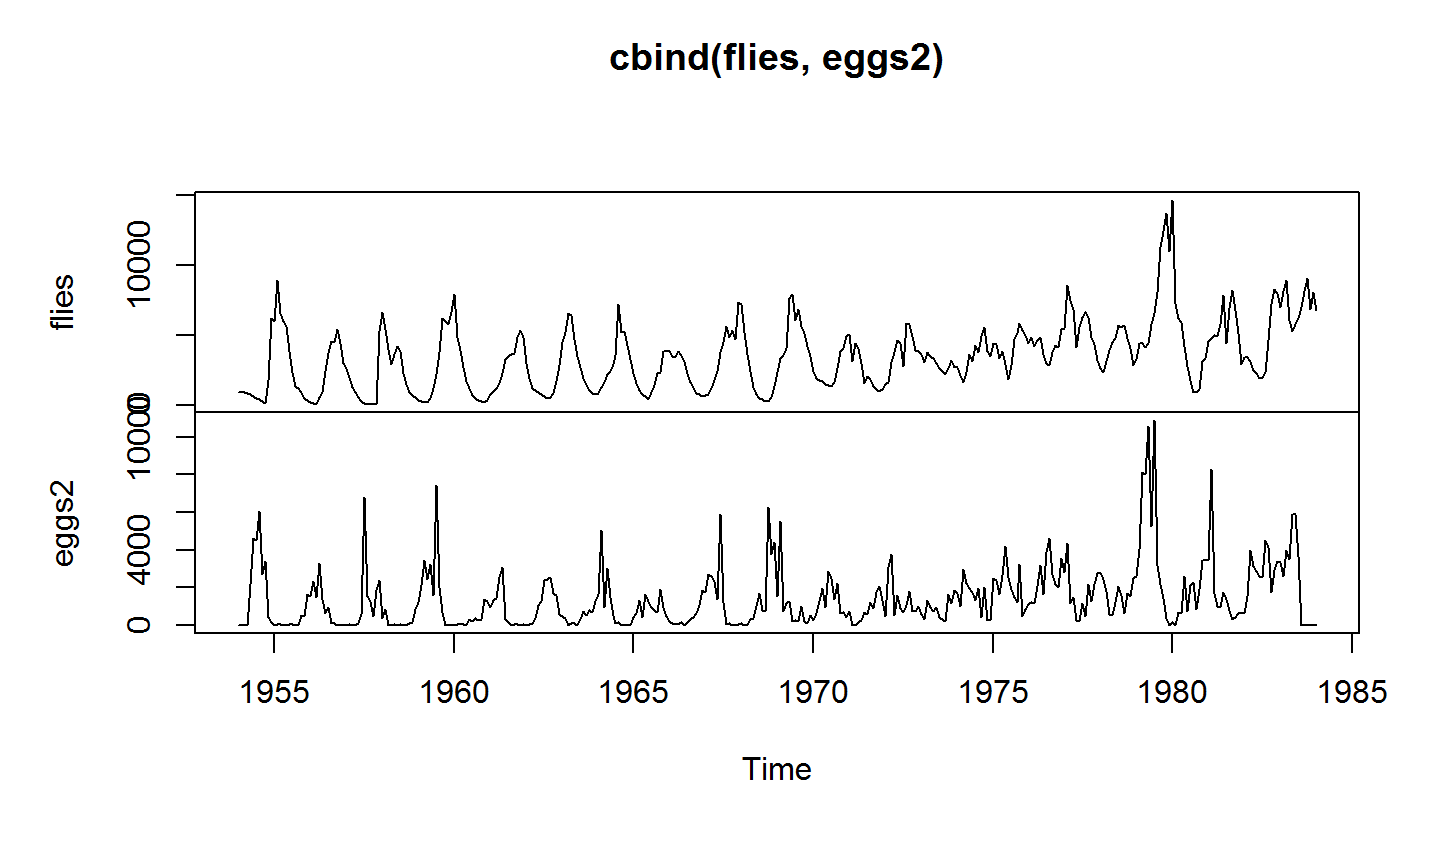
\includegraphics{simple_descriptive_techniques_files/figure-latex/unnamed-chunk-11-1.pdf}
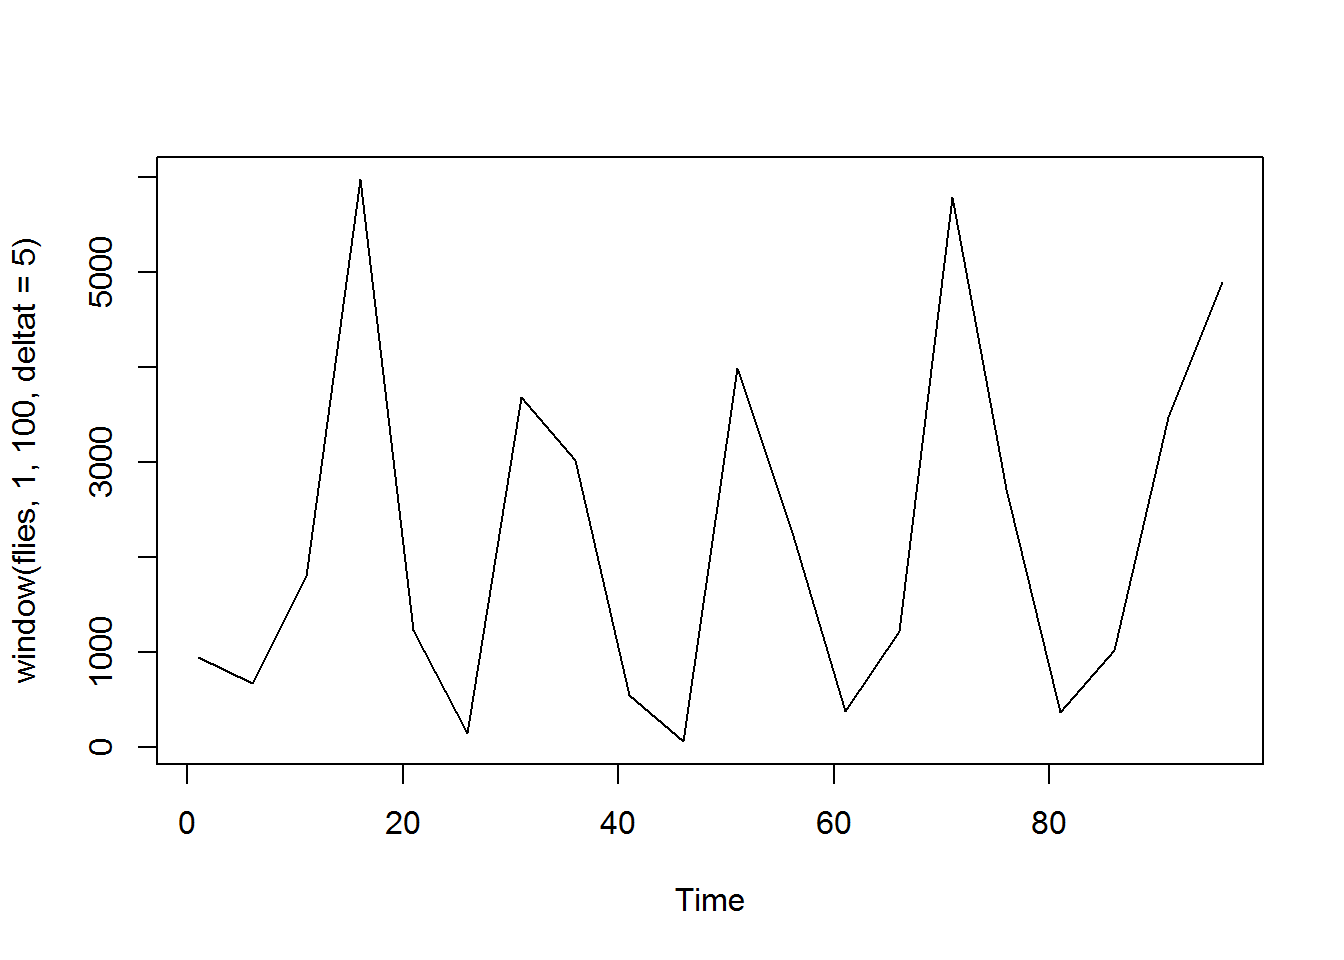
\includegraphics{simple_descriptive_techniques_files/figure-latex/unnamed-chunk-11-2.pdf}
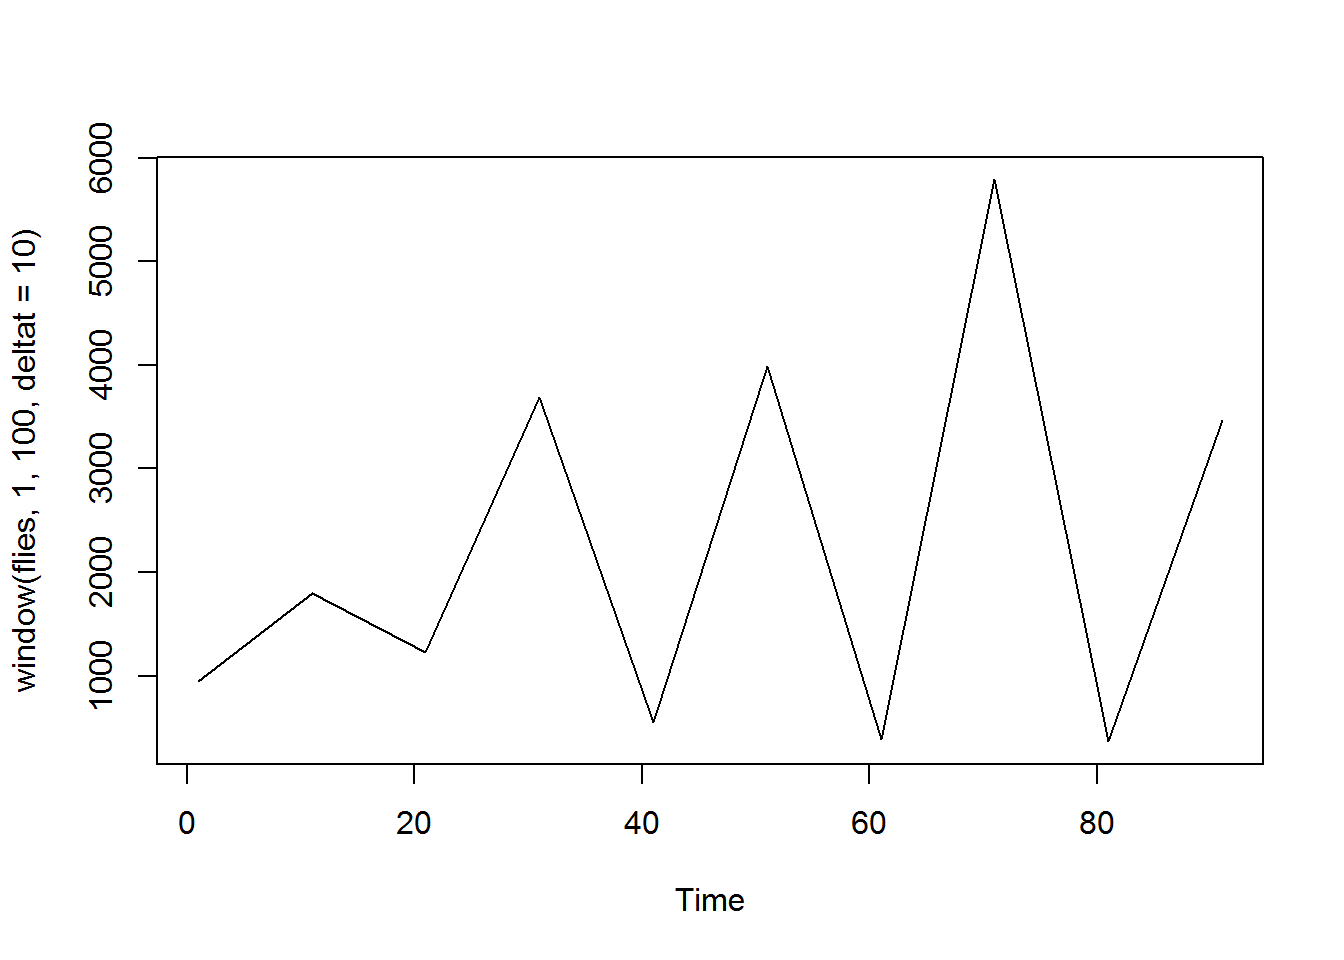
\includegraphics{simple_descriptive_techniques_files/figure-latex/unnamed-chunk-11-3.pdf}
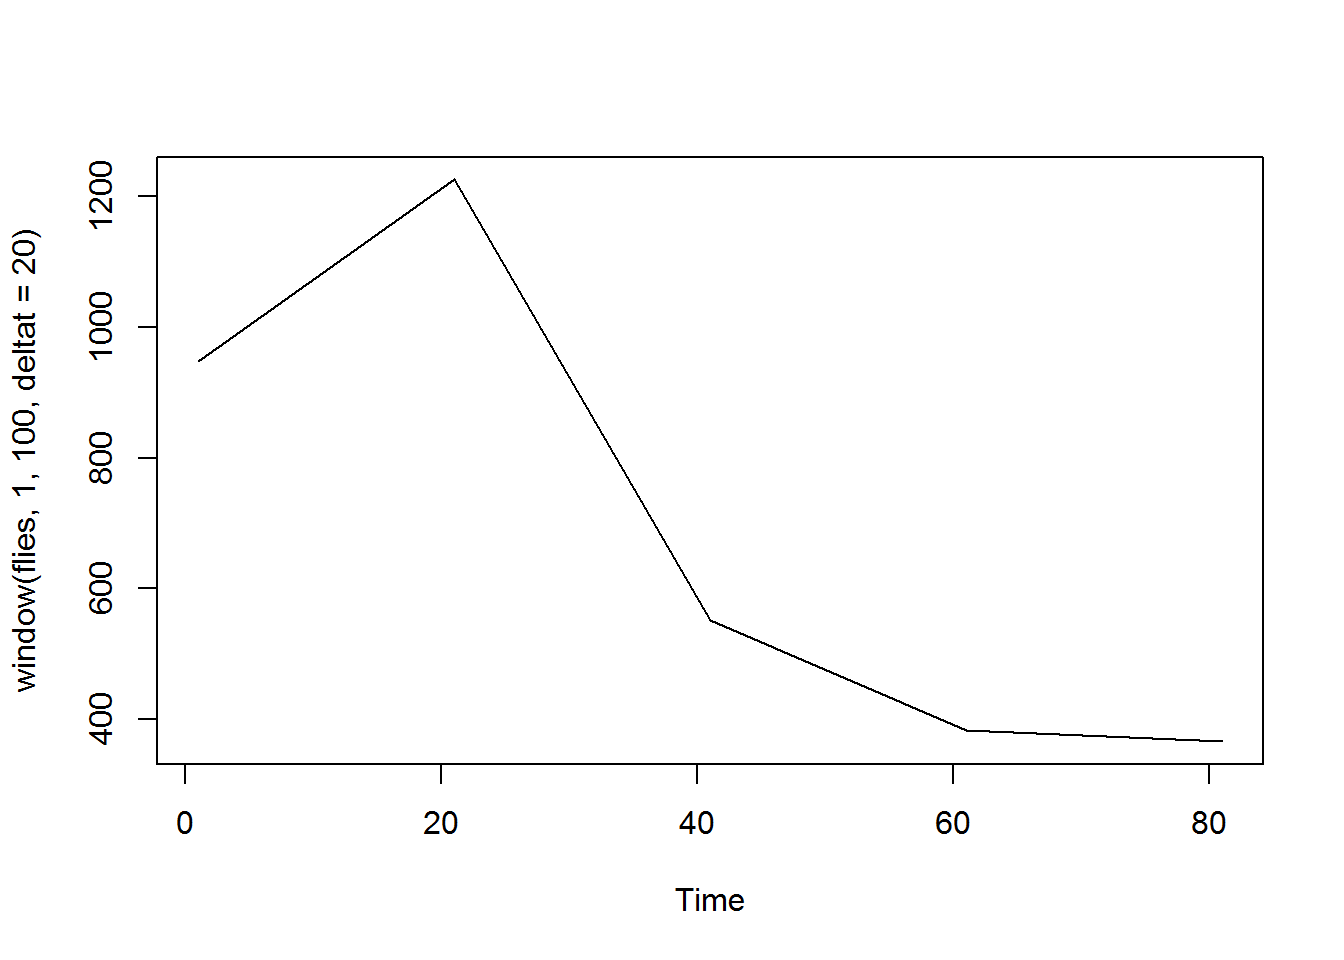
\includegraphics{simple_descriptive_techniques_files/figure-latex/unnamed-chunk-11-4.pdf}
\includegraphics{simple_descriptive_techniques_files/figure-latex/unnamed-chunk-11-5.pdf}
\includegraphics{simple_descriptive_techniques_files/figure-latex/unnamed-chunk-11-6.pdf}
\includegraphics{simple_descriptive_techniques_files/figure-latex/unnamed-chunk-11-7.pdf}
\includegraphics{simple_descriptive_techniques_files/figure-latex/unnamed-chunk-11-8.pdf}

\begin{verbatim}
## [[1]]
## NULL
## 
## [[2]]
## NULL
## 
## [[3]]
## NULL
## 
## [[4]]
## NULL
## 
## [[5]]
## NULL
## 
## [[6]]
## NULL
## 
## [[7]]
## NULL
## 
## [[8]]
## NULL
\end{verbatim}

\begin{Shaded}
\begin{Highlighting}[]
\KeywordTok{par}\NormalTok{(}\DataTypeTok{mfrow=}\KeywordTok{c}\NormalTok{(}\DecValTok{1}\NormalTok{,}\DecValTok{1}\NormalTok{))}
\end{Highlighting}
\end{Shaded}

This


\end{document}
